\chapter{Findings}
\label{ch:findings}

% * Repeatable, specific description
% * Provide intuition, key idea
% * State what the problem is that you want to address in that section
% * Describe all parts of life cycle: setup, run, maintenance, etc.
% * Explain with an example (together with the intuition and description, the scheme should have been explained 3 times from different perspectives)
% * Did we really fully explore the design space?
%     * Why are simpler solutions inappropriate?
%     * Explore design alternatives!
%     * Provide intuition on why certain design choices were taken, why alternatives were rejected
%     * Describe a strawman approach, show why it's inadequate

In this chapter we present the findings of our security analysis.
It is structured into two main sections:
The first section covers findings related to the SCION protocol in use.
The second section focuses on the Anapaya router itself.

\TODO{Update chapter with comments of Anapaya and updated findings}

\section{SCION Protocol}



\subsection{MAC Algorithm}
We compared the MAC algorithm used in the Anapaya version of SCION with the one available in the open source version.
Initially, we extracted the master secret from the file system and derived a MAC key in accordance with the definitions provided in the open source code.
Using this derived MAC key, we calculated the MAC value for a given hop field.
Our calculation matched the original MAC value, confirming the use of the open source MAC algorithm.
This algorithm, which is an AES-CMAC, is considered secure in terms of unforgeability.

In a discussion with Professor Perrig, it was highlighted that the master secret should be refreshed daily to maintain good cryptographic hygiene.
However, this practice is not followed on the Anapaya routers, as they consistently use the same master secret value.

Furthermore, we verified that the MAC value is being validated during transmission of a SCION packet.
Upon altering the MAC value or introducing unauthorized hop fields, the packet was correctly dropped by the Anapaya router.
This check ensures that no new path can be created, not even by combining it out of two valid ones.
Our tests confirmed the infeasibility of these manipulations.



\subsection{Source Authentication / DRKey}
Following the cryptographic analysis of the MAC algorithm, we examined another cryptographic related aspect of SCION: Source authentication based on DRKey.
This analysis turned out to be a short one, as we found that DRKey is not used in the SCION implementation on the Anapaya routers.
The lack of DRKey support enables various attacks on the SCION network.
For example, unauthenticated SCMP error messages can be injected into the network.
By sending an external interface down SCMP error message, an off-path attacker can possibly force retransmission of SCION packets on another path.



\subsection{Spoofing}
With the finding that the source is not authenticated, we investigated the possibility of spoofing the source information.
We altered the IP address as well as ISD-AS information and successfully transmitted the packet to the intended destination.
This demonstrates that no outbound filtering is active, allowing for source information spoofing.
If the destination application reverses the path information of the initial packet to send the reply, the response will return to the source AS rather than the spoofed one.
In the case of unidirectional paths or if the destination has a specific path policy defined, the destination may perform a path lookup based on the source information.
This scenario would result in a successful spoofing, where the spoofed location receives the packet.
Moreover, this can lead to reflection amplification attacks, particularly when the destination sends more data than the sender initially transmitted.
This can be exploited to launch denial-of-service attacks against the spoofed location.

We also attempted to force a path lookup at the recipient, assuming it would reverse the path information to reply.
The strategy involves using path segments that are about to expire.
The initial packet would use valid path segments, but when the destination reverses the path during the reply, the path segments would have already expired.
Depending on the application this could lead to a forced path lookup based on the spoofed source information, resulting in successful spoofing.
However, during our analysis, we observed that the Anapaya border router implementation drops network packets that have a path information that is going to expire in the next 30 seconds or less.
Unless an application requires more than 30 seconds to respond, a forced path lookup with nearly expired path information is prevented.

This is a significant divergence from the open-source implementation.
As illustrated in the pseudocode below, the open-source implementation only checks if the packet has expired based on the current time.
It does not account for the 30 additional seconds as observed in the Anapaya implementation.


\begin{lstlisting}[language={Go}, morekeywords={}, caption={Pseudocode of hop expiry check in open-source implementation of the border router.}, label={lst:hop-expiry}]
func (p *packetProcessor) (*@\textcolor{blue}{validateHopExpiry}@*)() (processResult, error) {
    expiration := util.SecsToTime(p.infoField.Timestamp).
        Add(path.ExpTimeToDuration(p.hopField.ExpTime))
    expired := expiration.Before(time.Now())
    if !expired {
        <move on with packet processing>
    }
    <drop packet + send SCMP packet with path expiry (*@error@*)>
}
\end{lstlisting}


To mitigate these vulnerabilities, we recommend adding egress source filtering to the border router implementation.
This measure would prevent malicious end hosts from performing such spoofing attacks.
Additionally, outbound filtering also directly enhances security for AS customers \cite[Section 7.7.3]{Perrig2022}, providing even higher incentives for ASes to perform egress filtering.
Source authentication is another effective solution to mitigate these attacks.
SPAO based on DRKey even provides source authentication on the first packet sent.
However, for this to be used, the DRKey feature must first be enabled by Anapaya.




\subsection{Path Extension}
For a spoofing or also denial-of-service attack, it is advisable to masquerade the source information; otherwise such a malicious source can be easily identified and blocked.
During our security analysis, we attempted to achieve this by altering and extending the SCION header.
As presented in the previous section, the source information can be spoofed.
Leveraging this knowledge, we modified the source to be a different (even made up) AS.
Additionally, we prepended the path header with extra hop fields and set the hop field index to the correct value.
These modifications make it appear as if the packet was sent by a customer of our AS.
The modified packet was successfully transmitted to the destination, which reverted the path information and sent the reply back to our AS.
This demonstrates that the path header can be extended with additional and invalid hop fields, allowing for the spoofing of the AS that originated the connection.
Implementing a simple check to filter packets with a hop field index set to zero (i.e., pointing to the first hop) for packets originated from AS-local end hosts would mitigate this issue.
However, this check does not protect against malicious ASes.
To address this threat, source authentication (e.g., SPAO) would be once again be an effective solution.
But again, this feature and DRKey are unfortunately not enabled in the Anapaya routers.

Given the ability to extend the path at will, we also assessed the impact of extending the path to the maximum length (i.e., 64 hop fields).
The destination must process and revert all these hops, which may lead to increased processing time and potentially result in a denial-of-service attack.
For this evaluation, 100 normal SCION pings were sent form the Kali machine in Zürich to the Anapaya router in Thun.
Additionally, 100 SCION pings with a modified path header containing the maximum number of hop fields were sent.
At the destination, the processing time was measured and is plotted in the following:

\begin{figure}[h]
    \centering
    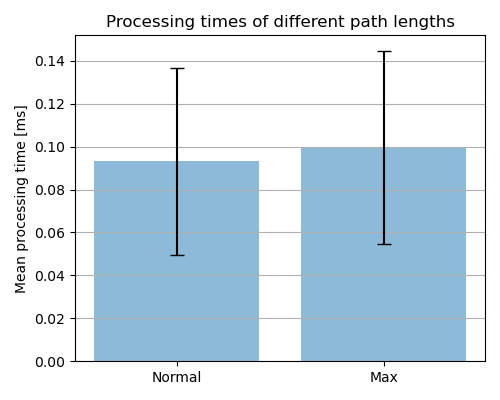
\includegraphics[width=0.75\textwidth]{processing_times_path_lengths.png}
    \caption{Processing times of a SCION ping with different path lengths.}
    \label{fig:path_extension}
\end{figure}

The results indicate that the processing time for the SCION pings with the maximum path length is slightly higher than for the normal SCION pings.
This simple evaluation demonstrates that the impact of extending the path to its maximum length is minimal and largely negligible.


\subsection{Path Header Modification}
This section addresses the modification of the path header by an on-path attacker rather than by the source.
This attack is also discussed in section 7.6.1 of the SCION book \cite{Perrig2022} and works as follows:
An attacker intercepts a SCION packet and modifies the path header by replacing path segments as desired.
The packet is then forwarded along the attacker chosen path rather than the original path intended by the sender.
These modifications can be reverted by the adversary in replies from the destination (e.g., when the destination inverts the path header to reply), making the sender unaware of the attack.
Our analysis within the CYD SCION network confirmed the feasibility of this attack.

To ensure that the selected path is actually used during transmission, the packet must be integrity protected.
A SCION built in solution would be the SCION packet authenticator option, but this feature is not enabled in the Anapaya routers.
Therefore, clients must implement their own solutions to ensure the integrity of the path header.
For instance, this can be achieved by adding a MAC to the entire packet or by comparing the path information of the received packet with the expected path information.






\section{Anapaya Router}
This section deals with the security related findings of the three operational Anapaya routers at the CYD Campus.
The devices run Ubuntu 22.04 as the operating system with Linux Kernel 5.15.0


\subsection{Secure Shell (SSH)}
The Anapaya routers are accessed via SSH with public key authentication and do not allow password authentication.
This is considered a robust security practice, as public key authentication is more secure than password authentication.
This is due to the higher entropy of key compared to passwords, and the fact that keys are not transmitted over the network.
However, our analysis identified some shortcomings with the SSH configuration that could be improved:

\begin{itemize}
    \item Various algorithms use elliptic curves cryptography (ECC) on curves that are believed to have been compromised by the National Security Agency (NSA) \cite{nist1_safecurves}.
    \item Some MAC algorithms use the broken SHA1 hash function, which potentially allows for collision attacks.
    \item The chacha20-poly1305@openssh.com cipher is enabled, which is susceptible to the Terrapin attack (CVE-2023-48795).
    This attack allows message prefix truncation, which enables an attacker to downgrade the security of a connection.
    \item A key exchange algorithm based on Diffie-Hellman group 14 is enabled. It uses a 2048-bit modulus, but only provides 112 bits of security.
    \item Some MAC algorithms are using the encrypt-and-MAC construction, which does not provide integrity of the ciphertext and can possibly leak information of the plaintext.
    It is recommended to use encrypt-then-MAC instead.
    \item Lastly, it should be noted that there are MAC algorithms enabled with a tag length of only 64 bits.
\end{itemize}

To improve the security of the SSH configuration, it is recommended to disable the aforementioned algorithms.
A detailed guide on implementing these changes can be found on this website \cite{sshauditHardeningGuides}.


Furthermore, it was found that the SSH server does not perform any rate limiting on login attempts.
Consequently, it is vulnerable to the DHEat denial of service attack \cite{dheatAttack}, where an attacker sends many Diffie-Hellman keys to the server, which then has to perform numerous expensive modular exponentiation and wasting CPU resources.
An attacker can also just send random big numbers, therefore avoiding computing valid keys.
Our experiments demonstrated that this attack could fully consume the CPU resources of the Anapaya routers in a matter of seconds.
However, due to the SCION dataplane's allocation on a dedicated CPU core, the impact on SCION functionality was minimal.
Nonetheless, other services, such as new SSH login attempts, experienced delays or were not even possible anymore.
To mitigate this attack, it is recommended to implement rate limiting on the SSH server, as it was shown in detail in this blog post \cite{dheatAnalysis}.


\subsection{Ubuntu Compliance}
By attempting to log in to the Anapaya routers via SSH, we observed that there is no banner displayed.
Banners usually contains a legal disclaimer that non-authorized access is prohibited and that activity may be monitored.
This can be crucial for legal compliance and for protecting the organization in the event of unauthorized access.
This is one of a few examples where the Anapaya router does not comply with the Ubuntu security guidelines.
In the following, we will discuss misconfigurations not complying with the CIS Ubuntu Linux 22.04 LTS audit \cite{cisUbuntuLinux2204LTS}.
Numbers in parentheses in this section refer to the corresponding section in the audit.

\begin{itemize}
    \item On two of the three examined routers, there is no password or other re-authentication needed to escalate privileges to root (5.2.4).
    \item While the systems are configured to only accept at least 6 characters long passwords, there is no password policy in place.
    For example, password complexity is not enforced (5.3.3.2.3) and also password reuse is not restricted (5.3.3.3.1).
    \item There is no shell timeout configured, which would log out an inactive user after a certain time (5.4.3.2).
    By setting a timeout, the risk of unauthorized access to the system can be reduced and also frees up resources associated with the idle session.
    \item Shared memory (the directory \texttt{/dev/shm}) can contain executable files, as the noexec option is not set (1.1.2.2.4).
    This option would prevent users from executing binaries from shared memory, which could be used to introduce malicious software into the system.
    \item The directories \texttt{/tmp} as well as \texttt{/var} are not mounted on separate partitions (1.1.2.1.1 and 1.1.2.4.1).
    Both directories are either world-writable or contain world-writable directories or files, which can be exploited to fill up the whole disk and impact the system's availability.
    Additionally, if the directories were mounted on separate partitions with the noexec option, it would prevent other attacks.
    For example an attacker could hard-link a system setuid binary to these locations and wait for it to be updated.
    After such an update, the hard-link would be broken and the attacker has its own copy of the setuid binary.
    If the binary has a security vulnerability it could be exploited to escalate privileges.
    \item There is no separate partition for the \texttt{/home} directory (1.1.2.3.1).
    Again, a user can fill up the disk and impact the system's availability.
    \item The permissions on crontab files are misconfigured (2.4.1.2 - 2.4.1.8) and can be read by unauthorized users.
    These files contain information about scheduled jobs, thus allowing an attacker to gain information about system jobs and potentially exploit them to escalate privileges.
    \item USB storage devices are not restricted (1.1.1.8) and therefore increases the physical attack surface.
    It can be misused to introduce malicious software into the system or to exfiltrate data.
    \item The SSH \texttt{LoginGraceTime} parameter is slightly set too high (5.2.13).
    This parameter specifies the time in seconds that the server allows for a successful login before disconnecting.
    A shorter time would reduce the risk of brute force attacks.
    Currently, the parameter is set to 120 seconds, but it is recommended to set it to 60 seconds.
    \item Root SSH login is enabled (5.2.20).
    By disabling root login over SSH, forces users to authenticate with their own account and then escalate privileges to root.
    This provides a clear audit trail and limits non-repudiation.
\end{itemize}


There are more compliance mismatches found during the audit.
Mostly related to ensure clear audit trails, including monitoring and logging of security-relevant events, or to disable unnecessary kernel modules
The full list of findings can be found \cref{app:automated-scan-result}.

\subsection{Security of systemd Services}
As seen in the previous section, the routers operating system can be optimized to ensure a higher level of security.
In this section, we will focus on the security of the systemd services running on the Anapaya routers.

For this purpose, we analyzed the services by running the \texttt{systemd-analyze security} command.
It evaluates the security settings and provides a score for each systemd service
This score is calculated based on the security features enabled for the service.
A higher score indicates a more exposed and potentially less secure service, whereas it only scores the configuration of the service.

The command can also be run on a single service, which then provides a detailed report on how the score was calculated.
In the following the output of the command and the scoring of the individual services is shown.


\TODO{Maybe try to add emojis here to output}

\begin{lstlisting}[language=bash, deletekeywords={local}, numbers=none, caption={Output of \texttt{systemd-analyze security}}]
$ systemd-analyze security
UNIT                                  EXPOSURE PREDICATE 
ModemManager.service                       6.3 MEDIUM    
appliance-controller.service               9.6 UNSAFE    
appliance-installer.service                9.6 UNSAFE    
apport.service                             9.6 UNSAFE    
caddy.service                              8.8 EXPOSED   
cloud-init-hotplugd.service                9.6 UNSAFE    
containerd.service                         9.6 UNSAFE    
cron.service                               9.6 UNSAFE    
dbus.service                               9.5 UNSAFE    
dm-event.service                           9.5 UNSAFE    
dmesg.service                              9.6 UNSAFE    
docker.service                             9.6 UNSAFE    
emergency.service                          9.5 UNSAFE    
getty@tty1.service                         9.6 UNSAFE    
irqbalance.service                         6.2 MEDIUM    
iscsid.service                             9.5 UNSAFE    
lvm2-lvmpolld.service                      9.5 UNSAFE    
lxd-agent.service                          9.5 UNSAFE    
multipathd.service                         9.5 UNSAFE    
networkd-dispatcher.service                9.6 UNSAFE    
open-vm-tools.service                      9.5 UNSAFE    
packagekit.service                         9.6 UNSAFE    
plymouth-start.service                     9.5 UNSAFE    
polkit.service                             9.6 UNSAFE    
rc-local.service                           9.6 UNSAFE    
rescue.service                             9.5 UNSAFE    
resolvconf.service                         9.5 UNSAFE    
rsyslog.service                            9.6 UNSAFE    
serial-getty@ttyS0.service                 9.6 UNSAFE    
snap.lxd.daemon.service                    9.6 UNSAFE    
snap.lxd.user-daemon.service               9.6 UNSAFE    
snapd.aa-prompt-listener.service           9.6 UNSAFE    
snapd.service                              9.6 UNSAFE    
ssh.service                                9.6 UNSAFE    
systemd-ask-password-console.service       9.4 UNSAFE    
systemd-ask-password-plymouth.service      9.5 UNSAFE    
systemd-ask-password-wall.service          9.4 UNSAFE    
systemd-fsckd.service                      9.5 UNSAFE    
systemd-initctl.service                    9.4 UNSAFE    
systemd-journald.service                   4.3 OK        
systemd-logind.service                     2.8 OK        
systemd-networkd.service                   2.9 OK        
systemd-resolved.service                   2.1 OK        
systemd-rfkill.service                     9.4 UNSAFE    
systemd-timesyncd.service                  2.1 OK        
systemd-udevd.service                      6.9 MEDIUM    
thermald.service                           9.6 UNSAFE    
ubuntu-advantage.service                   9.6 UNSAFE    
udisks2.service                            9.6 UNSAFE    
upower.service                             2.4 OK        
user@1000.service                          9.4 UNSAFE    
uuidd.service                              4.6 OK        
vgauth.service                             9.5 UNSAFE    
\end{lstlisting}

As one can see, many services are considered unsafe.
It is recommended to either disable unused services or to harden the configuration of the services to minimize the attack surface.

For example the \texttt{open-vm-tools} and \texttt{vgauth} services are related to VMware, but as on the routers no virtual machine is being used, these services can be disabled.
Also, the \texttt{ModemManager} service is not needed, as the router is not a modem and does not use mobile broadband (e.g., 2G/3G/4G) connections.
Furthermore, since the routers do not use WiFi or Bluetooth, also the \texttt{systemd-rfkill} service can be disabled.
Ubuntu Advantage is a subscription service that provides additional security features, such as livepatching, compliance checks, technical support and more.
As the Anapaya routers are not connected to the internet and are updated out-of-band, the \texttt{ubuntu-advantage} service is not needed and can be disabled.

Finally, it is also worth taking a closer look if the services can be configured more strictly.
Time did not permit to take a deep dive into the functionality of the services of the \texttt{appliance-controller} and \texttt{appliance-installer} of Anapaya.
However, the high exposure score of 9.6 indicates that these services were not configured to minimize the attack surface.
They enjoy a high level of capabilities and practically no restrictions.
We recommend reviewing the services and to restrict the rights to the minimum required for the services to function properly.


\subsection{Vulnerabilities}


In addition to ensuring the secure configuration of systemd services, it is also crucial to keep the software up-to-date.
This section provides an overview of vulnerabilities identified in the software running on the Anapaya routers.
The vulnerabilities were identified using a Nessus scan and are based on the software version and the Nessus CVE database.

Most identified weaknesses require local access to the system for exploitation.
Vulnerable versions of several software packages were found on the three devices, including \texttt{bash}, \texttt{vim}, \texttt{less}, \texttt{perl}, \texttt{git}, \texttt{tar}, \texttt{Intel Microcode}, \texttt{glibc}, and \texttt{libarchive}.
Some kernel vulnerabilities were also detected, but these require a local privileged attacker (e.g., one with CAP\_NET\_ADMIN capabilities) to exploit them.
The impact of these vulnerabilities ranges from denial of service attacks caused by system crashes to internal information leakage, to privilege escalation.

However, some vulnerabilities were identified that could be exploited remotely.
There are critical vulnerabilities associated with the drivers of the Intel Ethernet controller, which may allow an unauthenticated user to escalate privileges via network access (see CVE-2023-25775 and CVE-2023-45871 for more details).
Although some packages installed on the routers are vulnerable and could be exploited remotely, these packages are not actively used or running on the routers.
It is recommended to either update the affected packages or, preferably, remove unused software entirely to further reduce the attack surface.

A detailed report on all identified vulnerabilities can be found in \cref{app:automated-scan-result}.



\subsection{Docker}
% libc6 libssl1.1 openssl 1.1.1k

The individual services of the Anapaya router are containerized using Docker.
We conducted an automated and manual analysis of these containers to identify potential vulnerabilities.
The Docker images are based on Google's distroless Debian 11.1 base image \cite{githubGitHubGoogleContainerToolsdistroless}.
Such distroless images include only the necessary dependencies and omit a full operating system, which reduces the attack surface and enhances security.
However, our analysis revealed that this base image still contains unused binaries, such as \texttt{openssl}, its corresponding library \texttt{libssl}, and \texttt{c\_rehash}.
Furthermore, these binaries are outdated and vulnerable to various security threats, including command injection, use-after-free, double free, and denial of service attacks.
To improve the security of these Docker containers, it is recommended to remove these unused binaries by switching to the no-ssl variant of the distroless image (see \cite{githubGitHubGoogleContainerToolsdistroless}).

Further analysis of the libraries actually used to run the containers revealed that \texttt{libc} is outdated and has known vulnerabilities.
Although we were unable to directly exploit these vulnerabilities, it is recommended to update \texttt{libc} to the latest version to mitigate potential security threats.
Additionally, using the latest version of the Debian base image (currently version 12) is advisable.

Apart from the base image, it was observed that the live restore feature of Docker is not enabled.
Enabling this feature allows containers to continue running even if the Docker daemon is stopped during a crash or a planned update.
Without this feature, all running containers would stop if the daemon becomes unavailable, potentially leading to data loss and downtime for SCION services.
To ensure a higher availability of the SCION services, it is recommended to enable Docker's live restore feature.

Finally, to further improve availability, we suggest implementing resource limits for the Docker containers.
The inspected systems currently lack resource limits for the Docker containers.
Setting such limits would prevent a single container from consuming all the router's resources, potentially crashing it and impacting all SCION services.



\subsection{Management System}
Currently, no authentication is required for the CYD SCION users to access the Anapaya router's management web interface or management API.
Access is granted solely based on knowledge of the IP address of the border router.
This configuration allows users to make significant changes to the border router's configuration, including the following:

\begin{itemize}
    \item Altering firewall rules
    \item Reading and modifying SCION the forwarding key, which is used in the MAC calculations
    \item Changing DNS and NTP server settings
    \item Adding new TRCs
    \item Completely disabling the router
    \item Adding custom authentication options and potentially lock out other users from accessing the management system
\end{itemize}

This lack of authentication was also present on the test device, which shows that no default authentication is set up.
This observation is consistent with the official Anapaya documentation, which states that basic authentication is disabled by default \cite{anapayaManagemenDoc}.
To improve the security of the device and especially the SCION configuration, it is recommended to enable authentication for the management system.
We also encourage Anapaya to enable basic password authentication by default for newly deployed devices.


\subsection{Web Server}
The management system is also being served by a web server running on the router, accessible to any AS-local SCION user or any remote user in an AS with a configured SIG connection.
The web server in use is Caddy, version 2.6.4, released in February 2023.
This version is vulnerable to a denial of service attack known as Rapid Reset, which consumes the routers resources and eventually crashes it, thereby taking down all its services, including SCION.
The Rapid Reset attack exploits the HTTP/2 protocol's capability to open multiple streams within a single TCP connection.
An attacker can misuse this feature by simultaneously opening a large number of streams and then instantly closing them again.
By closing the streams right after opening, the attacker ensures that the number of active streams never exceed the limit allowed by the server.
Nonetheless, the server still has to perform substantial work for these canceled requests, including allocating memory for a new stream, parsing the query, performing header decompression, and other tasks \cite{googleWorksNovel}.

By modifying the code in an existing proof-of-concept attack \cite{githubGitHubMicrictorhttp2rststream}, we were able to attack our Anapaya router and finally taking it down withing a few seconds.
Notably, this attack is effective even when the management system is configured with authentication, as the web server itself is not protected by it.

The recommended solution to mitigate this vulnerability is to update the Caddy web server to version 2.7.5 or later, which addresses the Rapid Reset attack \cite{githubReleasesCaddyservercaddy}.



\subsection{General Recommendations}
% Test device shipped at begging of May 2024:
% - software/system/installed v2.8.0  -> dating back to end of september 2023 (2023-09-27T08:26:15.248888+00:00")
% - appliance v0.34.1                 -> 2023-10-20T13:45:22.216754+00:00

It is crucial to keep the software up-to-date to mitigate potential security threats.
The Anapaya routers should be updated regularly to ensure that the latest security patches are applied.
In May 2024, CYD bought and received a new Anapaya Router.
The system and SCION software versions on this new device were outdated and contained the software releases of autumn 2023 (end of September and mid of October).
An improvement on Anapaya's side would be to ship the routers with a more recent software version, ideally the latest release.




\section{Impact Traditional Internet on SCION}
We analyzed the impact of the traditional Internet on CYD's SCION connection by running a volumetric denial-of-service attack.

\TODO{Plots, text, etc.}

